\documentclass[../piano_di_progetto.tex]{subfiles}

\begin{document}


\subsection{Modello incrementale}
\label{sub:incr}

Per garantire la qualità del prodotto e uno sviluppo corretto che risulterà conforme rispetto ai requisiti richiesti sul lungo periodo, il gruppo ha scelto l’\glossario{approccio
incrementale}, ovvero l’impiego di \glossario{rilasci} che mirano ad integrare nel sistema ogni volta una nuova funzionalità. Questo sistema permette di ridurre il rischio di fallimento ad ogni iterazione, producendo un nuovo valore.

Il modello di sviluppo incrementale permette di progredire tramite cicli di incremento, 
ripetuti fino a quando il prodotto non soddisferà i requisiti richiesti dal cliente. \\
Il ciclo di incremento risulta suddiviso nei seguenti passi:
\begin{enumerate}
    \item Pianificazione;
    \item Analisi dei requisiti;
    \item Progettazione;
    \item Implementazione;
    \item Test;
    \item Valutazione.
\end{enumerate}
Ogni ciclo di incremento permette lo sviluppo di una funzionalità aggiuntiva.
La priorità nell'implementazione viene data alle funzionalità con importanza maggiore, quindi tutte quelle funzionalità base richieste dal committente o le funzionalità che sono dipendenze di altre. 
Seguendo questo modello le funzionalità principali e più importanti vengono implementate per prime, inserendo in questo modo quelle meno significative in un sistema stabile. 
La ciclicità prevista dal modello incrementale facilita anche il versionamento del sistema,
tracciando modifiche nette al software.\\
L'iter che verrà seguito dal gruppo per ogni fase è il seguente:
\begin{itemize}
    \item Il gruppo fissa degli incrementi e le relative date di scadenze entro le quali l'incremento deve essere concluso.
    \item Il carico di lavoro viene suddiviso tra i membri del gruppo in base ai ruoli assegnati.
    \item Al termine dell'incremento verrà analizzato il lavoro svolto e se gli obbiettivi sono stati rispettati (fase di \emph{verifica}).
\end{itemize}

\begin{figure}[H]
    \centering
    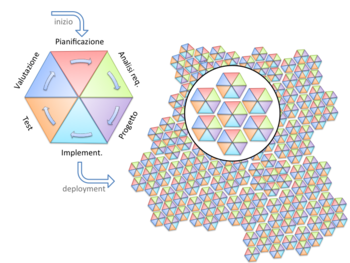
\includegraphics[scale = 0.6]{src/img/modello_incrementale.png}
    \caption{Rappresentazione del modello incrementale}
    \label{fig:logo}
\end{figure}

L'utilizzo di questo modello permette di ottenere importanti vantaggi, quali:
\begin{itemize}
    \item Maggior priorità alle funzionalità primarie, in questo modo possono essere sottoposte al cliente nel minor tempo possibile;
    \item Utilizzo dello sviluppo per incrementi successivi limita la modifica e le correzioni degli errori al singolo incremento, risultano meno onerose in termini di tempo e, di conseguenza, di costi;
    \item Le verifiche e i test sono circoscritti al singolo incremento, cioè alle nuove funzionalità;
    \item Possibilità di un maggior numero di feedback da parte del cliente, aumentando l'efficienza.
\end{itemize}

%TODO Allinenare incrementi in capitolo 3 - 4 - 5
\subsubsection{Incrementi individuati}
\label{ssub:incr_ind}

%Nei periodi di \emph{Progettezione architetturale} e \emph{Progettazione di dettaglio e codifica} sono stati individuati degli incrementi.
Di seguito viene riportato un tracciato incremento | Use case/requisito, in modo tale da comprendere più chiaramente gli UC o requisiti che verranno soddisfatti in ciascun incremento. 
%I requisiti riportati nella tabella includono tutti i requisiti figli. Tutti i requisiti non riporta-ti nella tabella sono da intendersi soddisfatti, in parte, da ogni incremento. Tali requisiti sonoreperibili all’interno del documentoAnalisi dei Requisiti.

Gli UC o i requisiti verranno sviluppati all'interno dell'incremento associato ad essi e verranno considerati soddisfatti in tutti gli incrementi successivi a quello di sviluppo. Gli UC e i requisiti qui riportati sono reperibili all'interno del documento \textsc{Analisi dei Requisiti}.
\begin{table}[!ht]
	\centering
	\begin{tabular}{|p{3cm}|p{3cm}|}
	\hline
	\rowcolor{lightgray}
    \textbf{Incremento} & \textbf{UC/Requisiti}\\
    \hline
    \rowcolor{lightgray}
	\multicolumn{2}{|p{6.44cm}|}{\textbf{Progettazione e codifica della technology baseline}}\\
    \hline
        Incremento I & RVO3\\
        Incremento II & RVO1\\
        Incremento III & UCW1.2  UCW3 \\
        Incremento IV & UCW2.2 UCW4.2.1 UCW4.2.2 UCW4.2.4 UCW4.2.5\\
        Incremento V & UCW1.3\\
    \hline
    \rowcolor{lightgray}
    \multicolumn{2}{|p{6.44cm}|}{\textbf{Progettazione e codifica di dettaglio}}\\
    \hline
        Incremento VI & UCS1\\ %implementazione fetch dati importati
        Incremento VII & UCW5.2.3\\ %implementazione funzionalità mancanti SPM
        Incremento VIII & UCW5.8 \\ %implementazione annullamento delle modifiche
        Incremento IX & UCW3.3 UCW5.4 UCW3.6  UCW5.5\\ %force field e distance map
        Incremento X & UCW4 UCW5.3\\ %implementazione modifiche
        Incremento XI & UCW3.4 UCW5.7\\ %heat map
        Incremento XII & UCW3.5 UCW5.6\\ %proiezione lineare multi asse
        Incremento XIII & UCW6 UCW7 UCW8 UCW9\\ %visualizzazione errori
        
    \hline	
	\end{tabular}
	\caption{Tabella tracciamento incremento-uc/requisiti}
\end{table}
%TODO eliminare incrementi non sviluppati in fase di RQ issue#116
\end{document}